
\documentclass[sigconf]{acmart}
\settopmatter{printacmref=false} % Removes citation information below abstract
\renewcommand\footnotetextcopyrightpermission[1]{} % removes footnote with conference information in first column
\pagestyle{plain} % removes running headers
  

\usepackage{wrapfig}
\usepackage{xcolor}
\usepackage{hyperref}
\hypersetup{
    colorlinks=true,
    linkcolor=blue,
    filecolor=magenta,      
    urlcolor=cyan,
}
\usepackage{listings}
\lstset{ 
    language=python,
    basicstyle=\small\color{black},
    keywordstyle=\color{black}\bfseries,                              
    frame=single, % adds a frame around the code
    captionpos=b, % sets the caption-position to bottom
    breaklines=true, % sets automatic line breaking
}
\usepackage[english]{babel}
\settopmatter{printfolios=true}
\setcopyright{none}

\begin{document}
\title{\HUGE{\textbf{Traind AI Warfleet}}}

\author{Michel Schwarz}
\affiliation{\institution{Hochschule Düsseldorf}}
\email{michel.schwarz@study.hs-duesseldorf.de}

\author{Niklas Tluk}
\affiliation{\institution{Hochschule Düsseldorf}}
\email{niklas.tluk@study.hs-duesseldorf.de}

\begin{abstract} % https://libguides.rhul.ac.uk/referencing/latex
The game War Fleet is a timeless classic, popular to this day in its countless iterations, ranging from the original board game to traditional video games and more recently VR applications. This is an implementation of said game in Python using neural networks and reinforcement learning. The A2C and PPO2 RL algorithms were employed to train intelligent agents, based on the OpenAI Gym toolkit and the OpenAI Baselines framework, to competently play it.

\end{abstract}
  
\begin{CCSXML}
<ccs2012>
   <concept>
       <concept_id>10010147.10010257.10010258.10010261</concept_id>
       <concept_desc>Computing methodologies~Reinforcement learning</concept_desc>
       <concept_significance>100</concept_significance>
       </concept>
   <concept>
       <concept_id>10010147.10010257.10010282.10010291</concept_id>
       <concept_desc>Computing methodologies~Learning from critiques</concept_desc>
       <concept_significance>100</concept_significance>
       </concept>
   <concept>
       <concept_id>10010147.10010178.10010219.10010221</concept_id>
       <concept_desc>Computing methodologies~Intelligent agents</concept_desc>
       <concept_significance>100</concept_significance>
       </concept>
   <concept>
       <concept_id>10010147.10010257.10010293.10010294</concept_id>
       <concept_desc>Computing methodologies~Neural networks</concept_desc>
       <concept_significance>100</concept_significance>
       </concept>
 </ccs2012>
\end{CCSXML}

\ccsdesc[100]{Computing methodologies~Reinforcement learning}
\ccsdesc[100]{Computing methodologies~Learning from critiques}
\ccsdesc[100]{Computing methodologies~Intelligent agents}
\ccsdesc[100]{Computing methodologies~Neural networks}

%% Keywords. The author(s) should pick words that accurately describe
%% the work being presented. Separate the keywords with commas.
\keywords{intelligent systems, intelligent agents, deep reinforcement learning, neural networks, A2C, PPO2}

%% A "teaser" image appears between the author and affiliation
%% information and the body of the document, and typically spans the
%% page.
%\begin{teaserfigure}
% 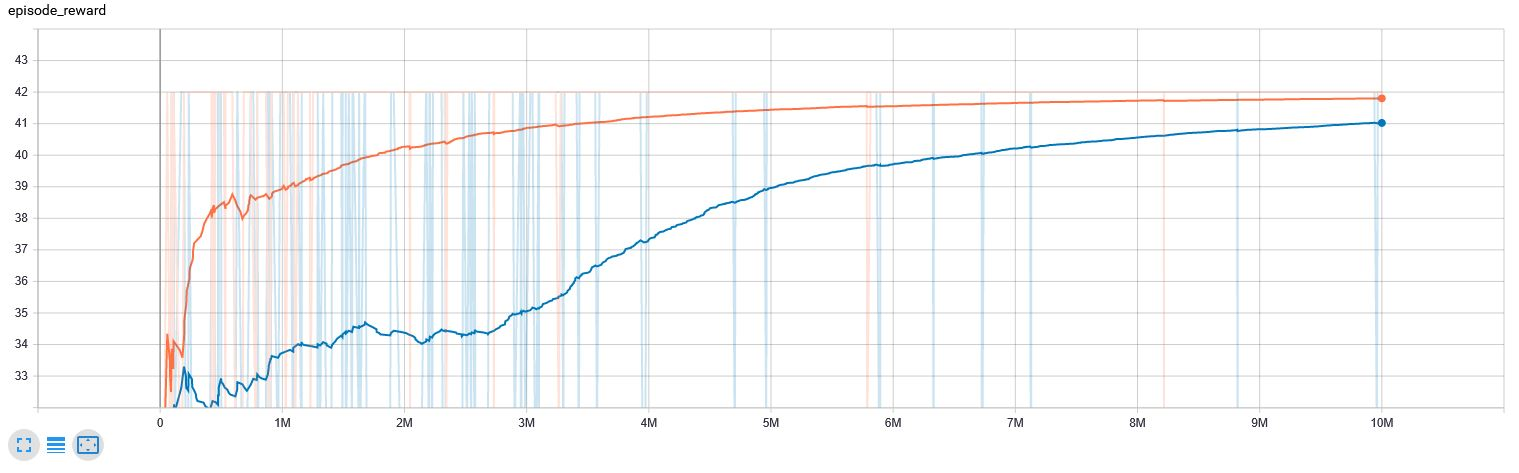
\includegraphics[width=\textwidth]{episode_reward_big} %placeholder
 % \caption{Episode Rewards A2C(Orange) and PPO2(Blue).}
%  \Description{}
 % \label{fig:teaser}
%\end{teaserfigure}

%%
%% This command processes the author and affiliation and title
%% information and builds the first part of the formatted document.
\maketitle 

\section{Introduction}
Considering the current prevalence of machine and deep learning intelligent systems are now more relevant than ever.
This project is part of our participation in the intelligent systems course at the HSD in Düsseldorf, Germany. The course served as an introduction to the design and implementation process of intelligent systems. It contained the history of machine learning, basic underlying principles, methods and algorithms aswell as current relevant topics in the media information field, like deep learning, date mining and predictive analytics. \\
\\
The Project files can be found \href{https://github.com/mickey175/Trained_Warfleet}{\textbf{\underline{here.}}} 

\section{Motivation}
Before starting this course we had already heard  about Deepmind's and OpenAI's impressive and at times even mind-boggling accomplishments with AlphaGO, AlphaStar, OpennAI Five and such. So when we were given the option to train an agent to play a simple game, using reinforcement learning and neural networks, ourselves we were excited and eagerly began coming up with ideas.

\section{Goal}
Our goal was the training of multiple intelligent agents, capable of competently playing the board game warfleet. 
We used python to implement the reinforcement learning process. 
To achieve that we implemented different reinforcement learning models. 

During the training the agent should show a significant improvement in playing the game.
The intermediate results should show that the agents are getting a rising reward.

At the end of the training the agent should be much better then the Computer.
The agent's enemy targets the ships using two random variables.
When the training is started, both started with random variables.
After a few played rounds it should turn out that the agent comprehends the structure and decide to attack a boat by its length an position on the battlefield. 
For example when a boat is hit at position (4/4) the agent should learn that the next field is left, right, up and down.
If the ship is not destroyed after two shots the agent should learn that the ship is longer than two fields.

\section{Environment}
To achieve this we also had to develop a feasible environment for the agent to be trained in. For this purpose we chose the OpenAI Gym toolkit, which provides an easy-to-use suite of reinforcement learning tasks.
The playing field or board of our game is a 10 by 10 2D array of the type integer. Possible values here are 1 for water, 2 for sections of a ship and 3 for shot positions(impacts).

\vspace{2.5mm} %2.5mm vertical space
\begin{lstlisting}[language=Python, caption=action\_space and observation\_space]
self.action_space = spaces.MultiDiscrete([10, 10])
self.observation_space = spaces.MultiDiscrete([
	[3, 3, 3, 3, 3, 3, 3, 3, 3, 3],
	[3, 3, 3, 3, 3, 3, 3, 3, 3, 3],
	[3, 3, 3, 3, 3, 3, 3, 3, 3, 3],
	[3, 3, 3, 3, 3, 3, 3, 3, 3, 3],
	[3, 3, 3, 3, 3, 3, 3, 3, 3, 3],
	[3, 3, 3, 3, 3, 3, 3, 3, 3, 3],
	[3, 3, 3, 3, 3, 3, 3, 3, 3, 3],
	[3, 3, 3, 3, 3, 3, 3, 3, 3, 3],
	[3, 3, 3, 3, 3, 3, 3, 3, 3, 3],
	[3, 3, 3, 3, 3, 3, 3, 3, 3, 3]
])

self.shot = "0"
self.empty_field = "1"
self.ship = "2"

    
\end{lstlisting}

\vspace{2.5mm}

%\begin{wrapfigure}{r}{}
% 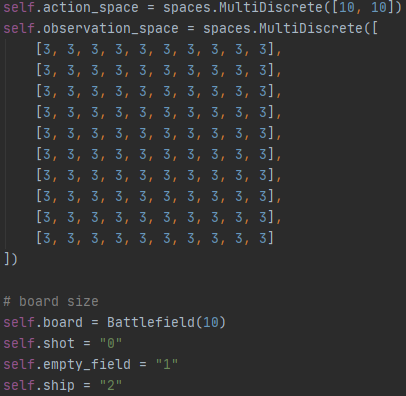
\includegraphics[width=40mm]{spaces.png}
%  \caption{Game Board, Observation and Action Space.}
%  \Description{...}
%  \label{fig:spaces}
%\end{wrapfigure}

The action space in our environment consists of all possible coordinates in said board while the observation space describes the amount of possible values, 3 in this case, for every board position.\\

\newline
When the game begins, the ships will be placed on the battlefield.
Each player has ten ships. Table 1 shows which ships are placed before the game begins. A method which is called place\_ships contains the code for the placement. This method is activated before the trained agent is activated. This means that the algorithms PPO2 and A2C are not related to the placement of the ships but only deal with the gameplay.

\begin{table}[htb]
\vspace{2.5mm}
\begin{tabular}{|c|c|c|ll}
\cline{1-3}
\textbf{Ship} & \textbf{Size} & \textbf{Quantity} \\ \cline{1-3}
small\_ship   & 2    & 4        \\ \cline{1-3}
middle\_ship  & 3    & 2        \\ \cline{1-3}
big\_ship     & 4    & 2        \\ \cline{1-3}
cruiser\_ship & 5    & 2        \\ \cline{1-3}
\end{tabular}
\vspace{2.5mm}
\caption{\label{tab:table-name}Ship information}
\end{table}

The following code is the console output for the Agent battlefield after the game has started. 
Each ship is placed inside the battlefield. You can see that the ships represented by the number 2 are placed side by side. At the same time, care is taken to ensure that the ships do not lie on top of each other.\\

\begin{lstlisting}[language=Python, caption=Battlefield in start condition]
--- Player/Agent Battlefield ---
[1, 1, 1, 1, 1, 1, 1, 1, 1, 1]
[1, 1, 1, 1, 1, 1, 1, 1, 1, 1]
[2, 2, 2, 2, 2, 1, 1, 1, 1, 1]
[2, 2, 2, 2, 2, 1, 1, 1, 2, 1]
[1, 2, 2, 1, 1, 1, 1, 1, 2, 1]
[1, 1, 1, 2, 2, 2, 1, 1, 1, 1]
[1, 1, 1, 2, 1, 2, 1, 1, 1, 1]
[1, 2, 1, 2, 1, 2, 2, 2, 2, 2]
[1, 2, 1, 1, 1, 2, 1, 1, 1, 1]
[1, 1, 2, 2, 2, 2, 1, 1, 1, 1]
\end{lstlisting}

\vspace{2.5mm}
After the battlefield is filled with ships, each player starts shooting.
A shot is visualized by the number 0. The code below shows the first line from the player/agent battlefield. The first shot is placed and the number 1 is replaced by the number 0.
\vspace{2.5mm}

\begin{lstlisting}[language=Python, caption=A line with a hit mark]
[1, 1, 1, 0, 1, 1, 1, 1, 1, 1]
\end{lstlisting}
\vspace{2.5mm}
Within the environment the ships of each player are listed in a list.
The list contains ship objects. A parameter contains the size for each ship. If a ship is hit by a shot, the size is reduced by 1, if the size is 0, the ship is removed from the list.
The game ends when one of these lists is empty.


\subsection{Reward}
The environment gives the agent a reward when the agent has hit a ship. 
This is a value of one for a simple hit, or ten if a whole ship is destroyed.
The agent should notice that the reward is significantly higher when a ship has sunk.


\vspace{2.5mm}
\section{Methods}
The Agent experience the environment by interacting with it. 
We trained out Agents without any given data-set. 
The Goal for the agent is to optimize its policy to receive as much reward as possible. 
Every time the agent got a reward the policy will increase the possibility to increase the probability of those actions.

The reinforcement learning algorithm are implemented in the stable-baselines project. Every algorithm has different characteristics.

\subsection{Procedure}
It should be clear how the agents interact with the environment and what is done to achieve the desired results.
The agent goes through the environment in several steps while the game is played in turns.

The current state of the environment is sent to the agent. Based on this state, the agent takes the next decision.
This decision is called action. In our case the agent receives the situation on the battlefield and can see if a target is hit or not.


\begin{figure}[ht]
 \centering
 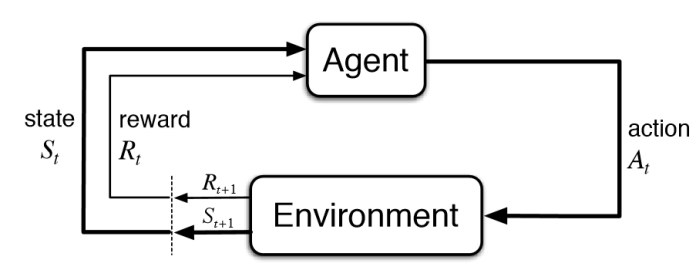
\includegraphics[width=50mm]{reinforcement-learning-fig1-700.jpg}
  \caption{Procedure}
  \label{fig:loss}
 %%% Source: https://www.kdnuggets.com/images/reinforcement-learning-fig1-700.jpg
\end{figure}

\subsection{Policy Gradient Methods}
To realize the training we need a Policy. To be able to process the tasks the agent needs a route that leads him to the target.
This Route is defined by a Policy. The agent is told by the policy what the next action will look like.
It is important to know that the policy is optimized on the basis of the self-generated data.\\

The Policy Gradient Methods is a bundle of reinforcement learning algorithms. The Goal is to solve reinforcement learning problems.
So the agent should learn a strategy which is increasingly improving. To achieve this, the reward should be increased to a maximum \cite[16-18]{ravichandiran2018hands}.
%[Policy REINFORCEMENT_LEARNING Zitat einfügen]

There are some default policies provided by the stable-baselines project. 
In our project we have used the MlpPolicy. MLP stands for Multilayer Perceptrons.
This type of network is called a feedforward network.
One layer is always connected to the next layer. So there is no path back.
The network consists of an input and an output layer. There can be several hidden layers between them \cite[174]{Frochte.2019}.
%[MLP Frochte Zitat einfügen]

Our learning methods are the Proximal Policy Optimization and Advantage Actor Critic.

\subsection{Proximal Policy Optimization}
The idea for PPO is similar to the TRPO method but it is not as complicated. 
PPO is a an on-policy Actor-Critic algorithm which means that the it is learning by its own generated data.
An important feature is that the algorithm pays more attention to the results of recently completed turns than to results that are significantly older.

\subsection{Advantage Actor-Critic}
 The A2C is an on-policy Actor-Critic algorithm. 
 It is based on the idea of the A3C but in a synchronized variant.
 In this case the critic is a value function that gives a feedback to the policy.
 The Policy is the actor. While the actor observes the environment, the critic estimates values to achieve a better action.
 This approach shows significant improvements in the results and is more and more used in policy gradient algorithms.
 
 %[Actor-Critic REINFORCEMENT_LEARNING Zitat einfügen]
 
\begin{figure}[ht]
 \centering
 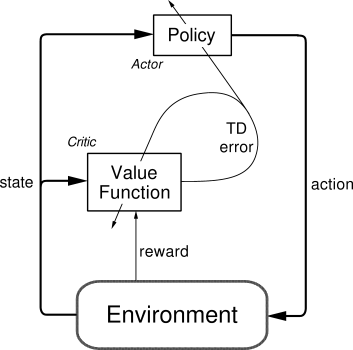
\includegraphics[width=50mm]{actor-critic.png}
  \caption{Actor-Critic principle}
  \label{fig:loss}
 %%% Source: http://incompleteideas.net/book/first/ebook/node66.html
\end{figure}
 

\section{Implementation}
The Open Ai Gym toolkit is imported to load our environment.
Before the learning process can start the environment is loaded.
To realize the implementation we imported some packages from stable-baselines. 
This toolbox makes it easy to implement reinforcement learning algorithms.
For beginners it is easy to start reinforcement learning by using those algorithms.

\vspace{2.5mm}

\begin{lstlisting}[language=Python, caption=Imports]
import gym
import gym_wf
from stable_baselines.common.policies import MlpPolicy
from stable_baselines.common.vec_env import DummyVecEnv
from stable_baselines import PPO2, A2C
\end{lstlisting}
\vspace{2.5mm} 
 
 \subsection{Algorithm implementation}
 The PPO2 algorithm is used with some different parameters to decrease the range between the policies.
 This process is called Hyperparameter tuning. 
 That means that the algorithm will be trained in a slightly different way by adjusting some parameters \cite[5-7]{schulman2017proximal}.
 % Zitat von Proximal Policy Optimization Algorithm PPO2 Paper
 
 \begin{lstlisting}[language=Python, caption=PPO2 implementation]
model = PPO2(MlpPolicy, env, verbose=1, 
tensorboard_log=log_dir, cliprange=0.1, 
gamma=0.99, ent_coef=0.001, vf_coef=0.2)

model.learn(total_timesteps=timesteps_input)
model.save(model_save)
 \end{lstlisting}
 \vspace{2.5mm}
 
 The A2C Algorithm is used without any parameters. 
 \begin{lstlisting}[language=Python, caption=A2C implementation]
model = A2C(MlpPolicy, env, 
verbose=1, tensorboard_log=log_dir)
model.learn(total_timesteps=timesteps_input)
model.save(model_save)
 \end{lstlisting}
 \vspace{2.5mm}
 
 \subsection{Training Settings}
 When the training starts, some information must be entered into the console.
 The first information is the algorithm that should be trained.
 The second is the number of timesteps.
 And the last one is the filename that contains the model.
 
\begin{lstlisting}[language=Python, caption=Console output before start]
Select algorithm (PPO2 or A2C only): PPO2
Choose number of timesteps: 10000000
Select model to test(input filename, eg. a2c_wf_2 or ppo2_wf_4):a2c_wf_3
\end{lstlisting}


\begin{figure*}
 \centering
  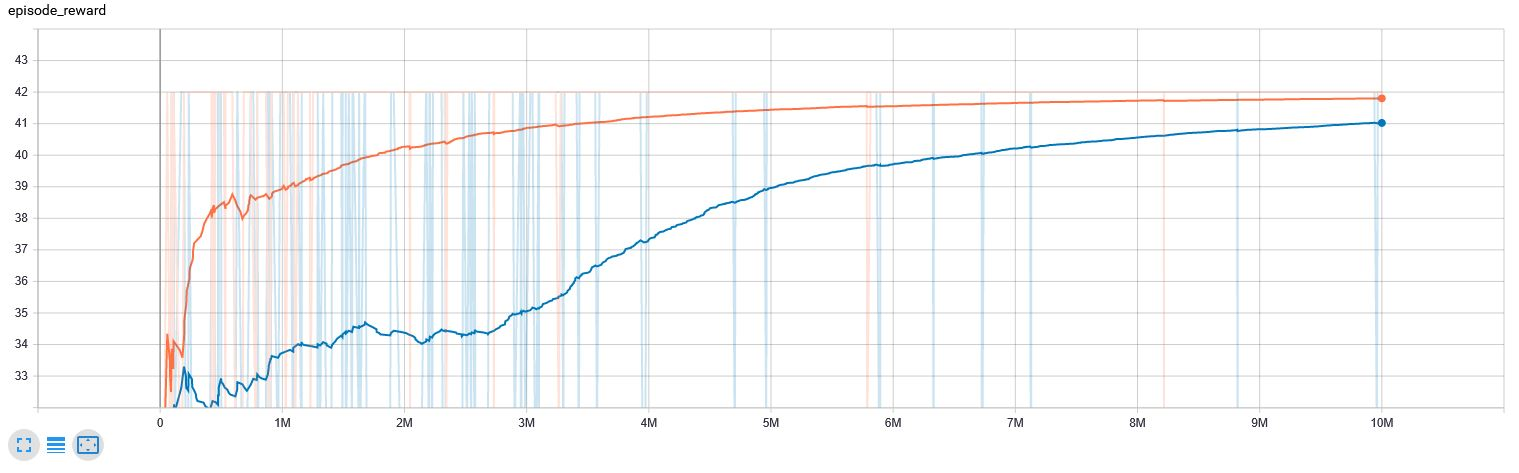
\includegraphics[width=\textwidth]{episode_reward_big} 
  \caption{Episode Rewards A2C(Orange) and PPO2(Blue).}
  \label{fig:reward1}
\end{figure*}
 
\section{Results}
The aforementioned training process resulted in the creation of multiple agents based on both algorithms. Through prolonged training the agents gained proficiency in playing the game, surpassing the random AI and finally reaching a win rate of 100\% with a varying number of its own ships remaining.
 \\
 \\
This is the end state of a War Fleet game played by the well trained ``a2c\_wp\_2 agents'' against a random AI:

\begin{lstlisting}[language=Python, caption=Computer battlefield end-state]
[0, 1, 0, 1, 0, 0, 0, 0, 0, 0]
[1, 1, 1, 1, 1, 1, 1, 1, 1, 1]
[0, 0, 0, 1, 0, 1, 1, 0, 0, 1]
[0, 0, 0, 1, 0, 0, 0, 0, 1, 1]
[1, 0, 1, 1, 0, 0, 0, 0, 1, 1] 
[0, 0, 1, 1, 0, 0, 0, 0, 1, 1] 
[0, 0, 0, 1, 0, 0, 1, 0, 0, 0] 
[0, 0, 0, 1, 0, 1, 1, 0, 1, 1] 
[0, 0, 0, 1, 1, 1, 1, 0, 0, 1] 
[1, 0, 0, 1, 0, 0, 0, 1, 0, 1] 
\end{lstlisting}
\\
\\
As you can see on the computer's battlefield, all of the its ships have been destroyed by our agent quite accurately with very little shots missing their mark .
\begin{lstlisting}[language=Python, caption=Agent battlefield end-state]
[0, 0, 0, 1, 1, 0, 0, 0, 1, 1]
[2, 2, 2, 0, 2, 0, 0, 1, 0, 1]
[0, 0, 0, 0, 1, 1, 0, 0, 0, 0] 
[1, 0, 1, 0, 0, 0, 1, 0, 0, 2]
[0, 0, 1, 2, 0, 0, 0, 2, 2, 2]
[0, 1, 0, 0, 0, 0, 0, 0, 0, 0]
[1, 0, 0, 2, 2, 1, 1, 1, 0, 0]
[0, 0, 0, 0, 2, 0, 0, 0, 0, 0]
[0, 0, 0, 0, 1, 0, 0, 0, 1, 0]
[0, 0, 0, 1, 1, 0, 0, 2, 0, 0]
\end{lstlisting}
Meanwhile the computer, with its random choices, didn't fare nearly as well. It only managed to sink 2 of our agents's ships, mostly just firing at the open water.
\\
\vfill
\begin{lstlisting}[language=Python, caption=Game information]
------------- End -------------
The Agent has won the game
Remaining Ships Computer: 0
Remaining Ships Agent: 8
Reward: [42.] /42
Turns: 121
\end{lstlisting}
\\
With 8 remeaning vessels our agent has bested its opponent in 121 turns, gaining a full reward of 42 points.
\\
Figure x1 shows a comparison of one agent of each type after a prolonged training of 10 million timesteps. It appears that the A2C based agent (a2c) learned very rapidly up to a certain point and than steadily improved over time more slowly while the PPO2 model (ppo2) slowly ramped up over time eventually reaching a steady rate of improvement and slowing down again when approaching the maximum possible reward. After only about 500.000 steps our A2C based model already earned a reward of around 38-39. Meanwhile our PPO2 agent was only able to again a reward of ~33 points.

\begin{figure}[ht]
 \centering
 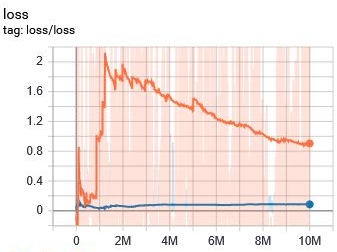
\includegraphics[width=80mm]{loss.png}
  \caption{Loss}
  \label{fig:loss}
\end{figure}
\\

At around 1.8 million time steps a2c came in with an average reward of about 40 points, thereafter steadily nearing the maximum reward of 42 points, while it took ppo2 around 6.5 million steps the achieve the same average.
\begin{figure}[ht]
 \centering
 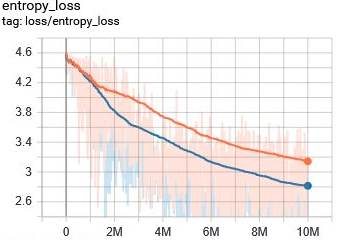
\includegraphics[width=80mm]{eloss.png}
  \caption{Loss}
  \label{fig:loss}
\end{figure}
\\
\\
\begin{figure*}
 \centering
  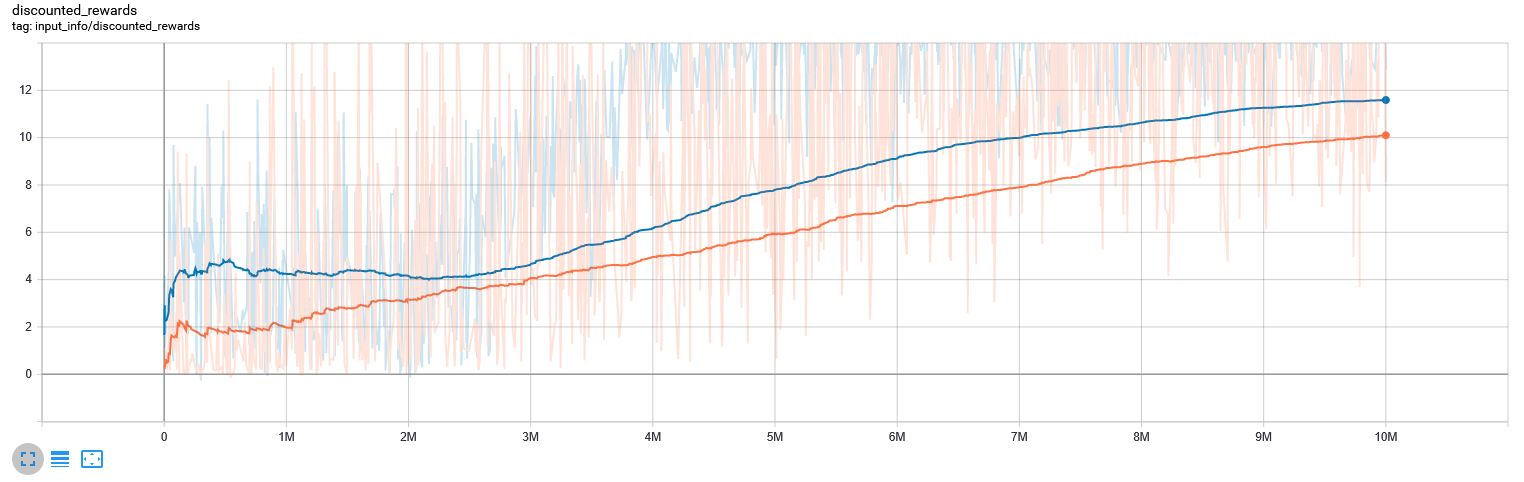
\includegraphics[width=\textwidth]{discounted_reward} 
  \caption{Discounted Rewards A2C(Orange) and PPO2(Blue).}
  \label{fig:reward2}
\end{figure*}

With the reward per episode(figure x1) and the discounted reward (figure x2) constantly increasing the loss (figure y1) and the entropy loss (figure y2) for a2c diminished over time after first spiking to a starting value of 2.1 and 4.5 respectively. While the entropy loss of ppo2 also decreased with further training its loss hovered at a value of ~0.1.

\vfill
\pagebreak
\section{Conclusion}
From those results we can conclude that our A2C based model is more suitable to our environment and was therefore able to gain a greater proficiency at playing the game than our PPO2 based approach at a rapid pace. 
   
\section{Future Work}
Currently there are no plans for further development, with leaves the future of  this project as uncertain. Some possible approaches are as follows. 
Different types of agents with varying amounts of training could be put up against each other to display the differences in learning efficiency etc. An option for users to face of against there trained agents could also be implemented.
\vfill
\pagebreak
\bibliographystyle{ieeetran}
\bibliography{bibtex_wf}
\end{document}
